%=========================================================
% BỔ SUNG BUỔI 4: hình học trong ngôi nhà + trò chơi mê cung
% Chèn bằng: %=========================================================
% BỔ SUNG BUỔI 4: hình học trong ngôi nhà + trò chơi mê cung
% Chèn bằng: %=========================================================
% BỔ SUNG BUỔI 4: hình học trong ngôi nhà + trò chơi mê cung
% Chèn bằng: %=========================================================
% BỔ SUNG BUỔI 4: hình học trong ngôi nhà + trò chơi mê cung
% Chèn bằng: \input{Data_PhieuBaiTap_HK0/Bo_Sung_Buoi_4}
% (đặt trong Buổi 4, trước dòng "--- Hết ---")
% Dùng các lệnh có sẵn: \OTdef, \OTcho, \OTbd, \OTo, \OTforma, \OTcham, màu OT...
%=========================================================

%---------- Hình nhỏ cho trò chơi (vẽ tại gốc tọa độ) ----------
% Chú ong (dài ~0,9cm)
\OTdef\OTong{%
  \filldraw[fill=cyan!20,draw=gray!60,thin] (-0.06,0.2) ellipse (0.11 and 0.19) (0.14,0.21) ellipse (0.1 and 0.17);
  \filldraw[fill=yellow!90!orange,draw=black!70,thin] (0,0) ellipse (0.36 and 0.22);
  \begin{scope}\clip (0,0) ellipse (0.36 and 0.22);
    \fill[black!80] (-0.14,-0.3) rectangle (-0.06,0.3);\fill[black!80] (0.04,-0.3) rectangle (0.12,0.3);\end{scope}
  \filldraw[fill=yellow!90!orange,draw=black!70,thin] (0.38,0.04) circle (0.12);
  \fill (0.42,0.07) circle (0.025);
  \draw[black!70,thin] (0.42,0.15)--(0.5,0.28) (0.35,0.15)--(0.37,0.29);
  \fill[black!80] (-0.38,0) -- (-0.5,0.03) -- (-0.38,-0.03) -- cycle;}
% Tổ ong
\OTdef\OTto{%
  \foreach \y/\w in {-0.45/0.5,-0.18/0.46,0.09/0.4,0.34/0.28}{\filldraw[fill=yellow!70!orange,draw=brown!70!black,rounded corners=3pt] (-\w,\y-0.14) rectangle (\w,\y+0.14);}
  \fill[brown!80!black] (0,-0.38) ellipse (0.14 and 0.1);
  \draw[brown!70!black,thin] (0,0.62)--(0,0.7);}
% Chú cá
\OTdef\OTca{%
  \filldraw[fill=orange!85!yellow,draw=orange!50!black,thin] (-0.1,0) ellipse (0.36 and 0.22);
  \filldraw[fill=orange!85!yellow,draw=orange!50!black,thin] (-0.4,0)--(-0.64,0.2)--(-0.64,-0.2)--cycle;
  \fill[white] (0.12,0.06) circle (0.06);\fill (0.14,0.06) circle (0.03);
  \draw[orange!50!black,thin] (-0.02,-0.15) .. controls (0.02,-0.05) .. (-0.02,0.1);}
% Thỏ
\OTdef\OTtho{%
  \foreach \s in {-1,1}{\filldraw[fill=white,draw=gray!60,thin] (0.1*\s+0.02,0.5) ellipse (0.07 and 0.22);\fill[pink!80] (0.1*\s+0.02,0.5) ellipse (0.03 and 0.14);}
  \filldraw[fill=white,draw=gray!60,thin] (0,-0.2) ellipse (0.3 and 0.26);
  \filldraw[fill=white,draw=gray!60,thin] (0.02,0.2) circle (0.2);
  \fill (-0.05,0.24) circle (0.025) (0.1,0.24) circle (0.025);
  \fill[pink!90!red] (0.02,0.16) circle (0.03);
  \filldraw[fill=white,draw=gray!60,thin] (-0.33,-0.25) circle (0.08);}
% Củ cà rốt
\OTdef\OTcarot{%
  \filldraw[fill=orange,draw=orange!60!black,thin] (-0.14,0.2)--(0.14,0.2)--(0,-0.4)--cycle;
  \draw[orange!60!black,very thin] (-0.07,0.1)--(0.03,0.1) (-0.04,-0.05)--(0.04,-0.05);
  \fill[green!55!black] (0,0.2) .. controls (-0.15,0.35) .. (-0.12,0.5) .. controls (-0.04,0.38) .. cycle;
  \fill[green!55!black] (0,0.2) .. controls (0.15,0.35) .. (0.12,0.5) .. controls (0.04,0.38) .. cycle;
  \fill[green!45!black] (0,0.2) .. controls (-0.04,0.4) .. (0,0.55) .. controls (0.04,0.4) .. cycle;}
% Ngôi sao vàng nhỏ
\OTdef\OTsao{\node[star,star points=5,star point ratio=2.3,inner sep=0pt,minimum size=0.4cm,draw=orange!70!black,fill=yellow,line width=0.4pt] at (0,0) {};}
% Lưới ô: \OTluoi{số cột}{rộng cm}{cao cm}{danh sách ô (theo hàng, từ trên xuống)}
\OTdef\OTluoi[4]{%
  \foreach \t [count=\k] in {#4}{%
    \pgfmathtruncatemacro{\cc}{mod(\k-1,#1)}\pgfmathtruncatemacro{\rr}{div(\k-1,#1)}%
    \node[draw=gray!70,fill=OTkem,rounded corners=4pt,line width=0.6pt,minimum width=#2cm,minimum height=#3cm,inner sep=0pt,font=\large] at ({#2*\cc},{-#3*\rr}) {\t};}}

%%%%%%%%%%%%%%%%%%%%%%%%%%%%%%%%%%%%%%%%%%%%%%%%%%%%%%%%%%
% Bài: đếm hình trong ngôi nhà
%%%%%%%%%%%%%%%%%%%%%%%%%%%%%%%%%%%%%%%%%%%%%%%%%%%%%%%%%%
\OTcho{7cm}\begin{bt}
    Đếm số hình trong bức tranh ngôi nhà rồi điền vào bảng.
    \OTbd{\centering
    \begin{tikzpicture}[scale=1.15]
        % nền cỏ
        \fill[green!35!white] (-0.6,-0.25) rectangle (5.9,0);
        \draw[green!50!black,thick] (-0.6,0)--(5.9,0);
        % ống khói (hình chữ nhật), vẽ trước mái
        \filldraw[fill=red!35!gray!60,draw=gray!70!black,thick] (1.75,2.9) rectangle (2.15,3.75);
        % thân nhà (hình vuông)
        \filldraw[fill=yellow!35!white,draw=brown!70!black,thick] (0,0) rectangle (2.4,2.4);
        % mái nhà (hình tam giác)
        \filldraw[fill=red!75!orange,draw=red!50!black,thick] (-0.2,2.4)--(1.2,3.6)--(2.6,2.4)--cycle;
        % cửa sổ tròn ở mái
        \filldraw[fill=cyan!25!white,draw=gray!70!black,thick] (1.2,2.95) circle (0.28);
        \draw[gray!70!black] (1.2,2.67)--(1.2,3.23) (0.92,2.95)--(1.48,2.95);
        % cửa ra vào (hình chữ nhật)
        \filldraw[fill=brown!60!orange,draw=brown!70!black,thick] (0.3,0) rectangle (0.9,1.3);
        \fill[yellow] (0.78,0.65) circle (0.04);
        % hai cửa sổ (hình vuông)
        \foreach \y in {0.6,1.5}{\filldraw[fill=cyan!25!white,draw=gray!70!black,thick] (1.3,\y) rectangle (2.0,\y+0.7);
          \draw[gray!70!black] (1.65,\y)--(1.65,\y+0.7) (1.3,\y+0.35)--(2.0,\y+0.35);}
        % cây (tam giác + chữ nhật)
        \filldraw[fill=brown!70!black!80,draw=brown!70!black,thick] (4.2,0) rectangle (4.6,1.0);
        \filldraw[fill=green!60!black!80,draw=green!40!black,thick] (3.6,1.0)--(5.2,1.0)--(4.4,2.8)--cycle;
        % mặt trời (hình tròn)
        \foreach \a in {0,30,...,330}{\draw[orange!80!yellow,thick,line cap=round] (4.7,3.8)+(\a:0.55)--+(\a:0.75);}
        \filldraw[fill=yellow,draw=orange!70!black,thick] (4.7,3.8) circle (0.45);
        % bảng thống kê
        \begin{scope}[shift={(6.8,3.3)}]
            \fill[OTnen] (0,0) rectangle (4.9,-0.65);
            \draw[line width=0.5pt] (0,0) rectangle (4.9,-3.05);
            \draw[line width=0.5pt] (2.4,0)--(2.4,-3.05);
            \foreach \i in {1,2,3,4}{\draw[line width=0.5pt] (0,-0.65-0.6*\i+0.6)--(4.9,-0.65-0.6*\i+0.6);}
            \node[font=\bfseries\small] at (1.2,-0.33) {Hình}; \node[font=\bfseries\small] at (3.65,-0.33) {Số lượng};
            \begin{scope}[shift={(1.2,-0.95)}]\filldraw[fill=gray!15,draw=gray!70] (0,0) circle (0.22);\end{scope}
            \begin{scope}[shift={(1.2,-1.55)}]\filldraw[fill=gray!15,draw=gray!70] (-0.22,-0.2) rectangle (0.22,0.24);\end{scope}
            \begin{scope}[shift={(1.2,-2.15)}]\filldraw[fill=gray!15,draw=gray!70] (-0.27,-0.2)--(0.27,-0.2)--(0,0.25)--cycle;\end{scope}
            \begin{scope}[shift={(1.2,-2.75)}]\filldraw[fill=gray!15,draw=gray!70] (-0.33,-0.17) rectangle (0.33,0.17);\end{scope}
        \end{scope}
    \end{tikzpicture}\par}
\end{bt}

%%%%%%%%%%%%%%%%%%%%%%%%%%%%%%%%%%%%%%%%%%%%%%%%%%%%%%%%%%
% Trò chơi 1: mê cung phép tính - giúp ong về tổ
%%%%%%%%%%%%%%%%%%%%%%%%%%%%%%%%%%%%%%%%%%%%%%%%%%%%%%%%%%
\OTcho{8.5cm}\begin{bt}
    \textbf{Trò chơi: Giúp ong về tổ.} Ong con chỉ bay qua những ô có kết quả bằng \textbf{12}. Em hãy tính nhẩm rồi tô màu đường bay của ong con về tổ nhé!
    \OTbd{\centering
    \begin{tikzpicture}
        \OTluoi{6}{2.15}{1.3}{{8+5},{14--3},{9+4},{18--6},{10+2},{17--5},
                              {5+7},{20--8},{16--5},{4+8},{6+7},{13--2},
                              {7+8},{9+3},{6+6},{15--3},{17--4},{5+9},
                              {18--5},{11+3},{15--6},{12+2},{19--8},{4+7}}
        \begin{scope}[shift={(-2.1,-1.3)},scale=1.5]\OTong\end{scope}
        \node[font=\bfseries\small] at (-2.1,-1.95) {Ong con};
        \begin{scope}[shift={(12.8,0)},scale=1.3]\OTto\end{scope}
        \node[font=\bfseries\small] at (12.8,-1.15) {Tổ ong};
    \end{tikzpicture}\par}
\end{bt}

%%%%%%%%%%%%%%%%%%%%%%%%%%%%%%%%%%%%%%%%%%%%%%%%%%%%%%%%%%
% Trò chơi 2: mê cung số tròn chục - cá con về biển
%%%%%%%%%%%%%%%%%%%%%%%%%%%%%%%%%%%%%%%%%%%%%%%%%%%%%%%%%%
\OTcho{7.5cm}\begin{bt}
    \textbf{Trò chơi: Cá con tìm kho báu.} Cá con bơi qua các ô ghi số tròn chục, đi theo thứ tự từ \textbf{bé đến lớn} (10, 20, 30, \ldots). Em hãy vẽ đường bơi giúp cá con nhé!
    \OTbd{\centering
    \begin{tikzpicture}
        \OTluoi{5}{2.3}{1.2}{{10},{20},{30},{12},{45},
                             {27},{63},{40},{50},{60},
                             {31},{58},{86},{19},{70},
                             {74},{9},{100},{90},{80}}
        \begin{scope}[shift={(-2.1,0)},scale=1.5]\OTca\end{scope}
        \node[font=\bfseries\small] at (-2.1,-0.7) {Cá con};
        \begin{scope}[shift={(4.6,-4.85)}]
            \node[star,star points=5,star point ratio=2.2,inner sep=0pt,minimum size=0.9cm,draw=orange!70!black,fill=yellow,line width=0.6pt] at (0,0) {};
            \node[font=\bfseries\small] at (0,-0.7) {Kho báu};
        \end{scope}
    \end{tikzpicture}\par}
\end{bt}

%%%%%%%%%%%%%%%%%%%%%%%%%%%%%%%%%%%%%%%%%%%%%%%%%%%%%%%%%%
% Trò chơi 3: mê cung thỏ tìm cà rốt, nhặt sao
%%%%%%%%%%%%%%%%%%%%%%%%%%%%%%%%%%%%%%%%%%%%%%%%%%%%%%%%%%
\OTcho{10cm}\begin{bt}
    \textbf{Trò chơi: Thỏ con tìm cà rốt.} Em hãy vẽ đường đi giúp thỏ con đến chỗ cà rốt. Trên đường đi, thỏ nhặt được những ngôi sao nào? Hãy đếm và điền số.
    \OTbd{\centering
    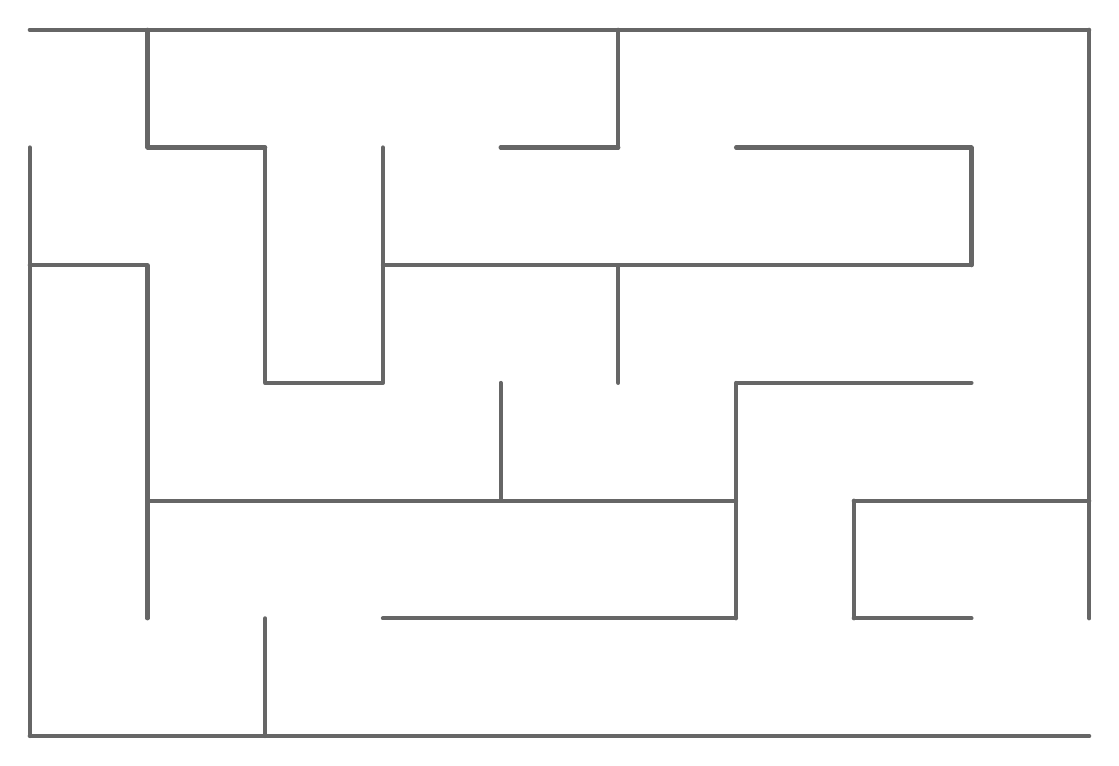
\begin{tikzpicture}[scale=1.3]
        \draw[line width=1.5pt,line cap=round,gray!80!black] (1.15,0.00)--(1.15,-1.15) (5.75,0.00)--(5.75,-1.15) (2.30,-1.15)--(2.30,-2.30) (3.45,-1.15)--(3.45,-2.30) (9.20,-1.15)--(9.20,-2.30) (1.15,-2.30)--(1.15,-3.45) (2.30,-2.30)--(2.30,-3.45) (3.45,-2.30)--(3.45,-3.45) (5.75,-2.30)--(5.75,-3.45) (1.15,-3.45)--(1.15,-4.60) (4.60,-3.45)--(4.60,-4.60) (6.90,-3.45)--(6.90,-4.60) (1.15,-4.60)--(1.15,-5.75) (6.90,-4.60)--(6.90,-5.75) (8.05,-4.60)--(8.05,-5.75) (2.30,-5.75)--(2.30,-6.90) (1.15,-1.15)--(2.30,-1.15) (4.60,-1.15)--(5.75,-1.15) (6.90,-1.15)--(8.05,-1.15) (8.05,-1.15)--(9.20,-1.15) (0.00,-2.30)--(1.15,-2.30) (3.45,-2.30)--(4.60,-2.30) (4.60,-2.30)--(5.75,-2.30) (5.75,-2.30)--(6.90,-2.30) (6.90,-2.30)--(8.05,-2.30) (8.05,-2.30)--(9.20,-2.30) (2.30,-3.45)--(3.45,-3.45) (6.90,-3.45)--(8.05,-3.45) (8.05,-3.45)--(9.20,-3.45) (1.15,-4.60)--(2.30,-4.60) (2.30,-4.60)--(3.45,-4.60) (3.45,-4.60)--(4.60,-4.60) (4.60,-4.60)--(5.75,-4.60) (5.75,-4.60)--(6.90,-4.60) (8.05,-4.60)--(9.20,-4.60) (9.20,-4.60)--(10.35,-4.60) (3.45,-5.75)--(4.60,-5.75) (4.60,-5.75)--(5.75,-5.75) (5.75,-5.75)--(6.90,-5.75) (8.05,-5.75)--(9.20,-5.75) (0.00,0.00)--(10.35,0.00) (0.00,-6.90)--(10.35,-6.90) (0.00,-1.15)--(0.00,-6.90) (10.35,0.00)--(10.35,-5.75);
        \foreach \x/\y in {1.72/-1.72, 2.88/-4.02, 5.17/-2.88, 6.33/-2.88, 8.62/-2.88, 8.62/-4.02, 7.47/-6.33, 8.62/-1.72, 8.62/-5.17, 6.33/-5.17}{\begin{scope}[shift={(\x,\y)}]\OTsao\end{scope}}
        \begin{scope}[shift={(-0.7,-0.58)},scale=1.1]\OTtho\end{scope}
        \begin{scope}[shift={(10.0,-5.75)},scale=1.3]\OTcarot\end{scope}
    \end{tikzpicture}\par}
    \par\medskip
    \noindent Thỏ con nhặt được tất cả \OTo\ ngôi sao trên đường đến chỗ cà rốt. \hfill Có \OTo\ ngôi sao ở các ngõ cụt (không nằm trên đường đi).
\end{bt}

% (đặt trong Buổi 4, trước dòng "--- Hết ---")
% Dùng các lệnh có sẵn: \OTdef, \OTcho, \OTbd, \OTo, \OTforma, \OTcham, màu OT...
%=========================================================

%---------- Hình nhỏ cho trò chơi (vẽ tại gốc tọa độ) ----------
% Chú ong (dài ~0,9cm)
\OTdef\OTong{%
  \filldraw[fill=cyan!20,draw=gray!60,thin] (-0.06,0.2) ellipse (0.11 and 0.19) (0.14,0.21) ellipse (0.1 and 0.17);
  \filldraw[fill=yellow!90!orange,draw=black!70,thin] (0,0) ellipse (0.36 and 0.22);
  \begin{scope}\clip (0,0) ellipse (0.36 and 0.22);
    \fill[black!80] (-0.14,-0.3) rectangle (-0.06,0.3);\fill[black!80] (0.04,-0.3) rectangle (0.12,0.3);\end{scope}
  \filldraw[fill=yellow!90!orange,draw=black!70,thin] (0.38,0.04) circle (0.12);
  \fill (0.42,0.07) circle (0.025);
  \draw[black!70,thin] (0.42,0.15)--(0.5,0.28) (0.35,0.15)--(0.37,0.29);
  \fill[black!80] (-0.38,0) -- (-0.5,0.03) -- (-0.38,-0.03) -- cycle;}
% Tổ ong
\OTdef\OTto{%
  \foreach \y/\w in {-0.45/0.5,-0.18/0.46,0.09/0.4,0.34/0.28}{\filldraw[fill=yellow!70!orange,draw=brown!70!black,rounded corners=3pt] (-\w,\y-0.14) rectangle (\w,\y+0.14);}
  \fill[brown!80!black] (0,-0.38) ellipse (0.14 and 0.1);
  \draw[brown!70!black,thin] (0,0.62)--(0,0.7);}
% Chú cá
\OTdef\OTca{%
  \filldraw[fill=orange!85!yellow,draw=orange!50!black,thin] (-0.1,0) ellipse (0.36 and 0.22);
  \filldraw[fill=orange!85!yellow,draw=orange!50!black,thin] (-0.4,0)--(-0.64,0.2)--(-0.64,-0.2)--cycle;
  \fill[white] (0.12,0.06) circle (0.06);\fill (0.14,0.06) circle (0.03);
  \draw[orange!50!black,thin] (-0.02,-0.15) .. controls (0.02,-0.05) .. (-0.02,0.1);}
% Thỏ
\OTdef\OTtho{%
  \foreach \s in {-1,1}{\filldraw[fill=white,draw=gray!60,thin] (0.1*\s+0.02,0.5) ellipse (0.07 and 0.22);\fill[pink!80] (0.1*\s+0.02,0.5) ellipse (0.03 and 0.14);}
  \filldraw[fill=white,draw=gray!60,thin] (0,-0.2) ellipse (0.3 and 0.26);
  \filldraw[fill=white,draw=gray!60,thin] (0.02,0.2) circle (0.2);
  \fill (-0.05,0.24) circle (0.025) (0.1,0.24) circle (0.025);
  \fill[pink!90!red] (0.02,0.16) circle (0.03);
  \filldraw[fill=white,draw=gray!60,thin] (-0.33,-0.25) circle (0.08);}
% Củ cà rốt
\OTdef\OTcarot{%
  \filldraw[fill=orange,draw=orange!60!black,thin] (-0.14,0.2)--(0.14,0.2)--(0,-0.4)--cycle;
  \draw[orange!60!black,very thin] (-0.07,0.1)--(0.03,0.1) (-0.04,-0.05)--(0.04,-0.05);
  \fill[green!55!black] (0,0.2) .. controls (-0.15,0.35) .. (-0.12,0.5) .. controls (-0.04,0.38) .. cycle;
  \fill[green!55!black] (0,0.2) .. controls (0.15,0.35) .. (0.12,0.5) .. controls (0.04,0.38) .. cycle;
  \fill[green!45!black] (0,0.2) .. controls (-0.04,0.4) .. (0,0.55) .. controls (0.04,0.4) .. cycle;}
% Ngôi sao vàng nhỏ
\OTdef\OTsao{\node[star,star points=5,star point ratio=2.3,inner sep=0pt,minimum size=0.4cm,draw=orange!70!black,fill=yellow,line width=0.4pt] at (0,0) {};}
% Lưới ô: \OTluoi{số cột}{rộng cm}{cao cm}{danh sách ô (theo hàng, từ trên xuống)}
\OTdef\OTluoi[4]{%
  \foreach \t [count=\k] in {#4}{%
    \pgfmathtruncatemacro{\cc}{mod(\k-1,#1)}\pgfmathtruncatemacro{\rr}{div(\k-1,#1)}%
    \node[draw=gray!70,fill=OTkem,rounded corners=4pt,line width=0.6pt,minimum width=#2cm,minimum height=#3cm,inner sep=0pt,font=\large] at ({#2*\cc},{-#3*\rr}) {\t};}}

%%%%%%%%%%%%%%%%%%%%%%%%%%%%%%%%%%%%%%%%%%%%%%%%%%%%%%%%%%
% Bài: đếm hình trong ngôi nhà
%%%%%%%%%%%%%%%%%%%%%%%%%%%%%%%%%%%%%%%%%%%%%%%%%%%%%%%%%%
\OTcho{7cm}\begin{bt}
    Đếm số hình trong bức tranh ngôi nhà rồi điền vào bảng.
    \OTbd{\centering
    \begin{tikzpicture}[scale=1.15]
        % nền cỏ
        \fill[green!35!white] (-0.6,-0.25) rectangle (5.9,0);
        \draw[green!50!black,thick] (-0.6,0)--(5.9,0);
        % ống khói (hình chữ nhật), vẽ trước mái
        \filldraw[fill=red!35!gray!60,draw=gray!70!black,thick] (1.75,2.9) rectangle (2.15,3.75);
        % thân nhà (hình vuông)
        \filldraw[fill=yellow!35!white,draw=brown!70!black,thick] (0,0) rectangle (2.4,2.4);
        % mái nhà (hình tam giác)
        \filldraw[fill=red!75!orange,draw=red!50!black,thick] (-0.2,2.4)--(1.2,3.6)--(2.6,2.4)--cycle;
        % cửa sổ tròn ở mái
        \filldraw[fill=cyan!25!white,draw=gray!70!black,thick] (1.2,2.95) circle (0.28);
        \draw[gray!70!black] (1.2,2.67)--(1.2,3.23) (0.92,2.95)--(1.48,2.95);
        % cửa ra vào (hình chữ nhật)
        \filldraw[fill=brown!60!orange,draw=brown!70!black,thick] (0.3,0) rectangle (0.9,1.3);
        \fill[yellow] (0.78,0.65) circle (0.04);
        % hai cửa sổ (hình vuông)
        \foreach \y in {0.6,1.5}{\filldraw[fill=cyan!25!white,draw=gray!70!black,thick] (1.3,\y) rectangle (2.0,\y+0.7);
          \draw[gray!70!black] (1.65,\y)--(1.65,\y+0.7) (1.3,\y+0.35)--(2.0,\y+0.35);}
        % cây (tam giác + chữ nhật)
        \filldraw[fill=brown!70!black!80,draw=brown!70!black,thick] (4.2,0) rectangle (4.6,1.0);
        \filldraw[fill=green!60!black!80,draw=green!40!black,thick] (3.6,1.0)--(5.2,1.0)--(4.4,2.8)--cycle;
        % mặt trời (hình tròn)
        \foreach \a in {0,30,...,330}{\draw[orange!80!yellow,thick,line cap=round] (4.7,3.8)+(\a:0.55)--+(\a:0.75);}
        \filldraw[fill=yellow,draw=orange!70!black,thick] (4.7,3.8) circle (0.45);
        % bảng thống kê
        \begin{scope}[shift={(6.8,3.3)}]
            \fill[OTnen] (0,0) rectangle (4.9,-0.65);
            \draw[line width=0.5pt] (0,0) rectangle (4.9,-3.05);
            \draw[line width=0.5pt] (2.4,0)--(2.4,-3.05);
            \foreach \i in {1,2,3,4}{\draw[line width=0.5pt] (0,-0.65-0.6*\i+0.6)--(4.9,-0.65-0.6*\i+0.6);}
            \node[font=\bfseries\small] at (1.2,-0.33) {Hình}; \node[font=\bfseries\small] at (3.65,-0.33) {Số lượng};
            \begin{scope}[shift={(1.2,-0.95)}]\filldraw[fill=gray!15,draw=gray!70] (0,0) circle (0.22);\end{scope}
            \begin{scope}[shift={(1.2,-1.55)}]\filldraw[fill=gray!15,draw=gray!70] (-0.22,-0.2) rectangle (0.22,0.24);\end{scope}
            \begin{scope}[shift={(1.2,-2.15)}]\filldraw[fill=gray!15,draw=gray!70] (-0.27,-0.2)--(0.27,-0.2)--(0,0.25)--cycle;\end{scope}
            \begin{scope}[shift={(1.2,-2.75)}]\filldraw[fill=gray!15,draw=gray!70] (-0.33,-0.17) rectangle (0.33,0.17);\end{scope}
        \end{scope}
    \end{tikzpicture}\par}
\end{bt}

%%%%%%%%%%%%%%%%%%%%%%%%%%%%%%%%%%%%%%%%%%%%%%%%%%%%%%%%%%
% Trò chơi 1: mê cung phép tính - giúp ong về tổ
%%%%%%%%%%%%%%%%%%%%%%%%%%%%%%%%%%%%%%%%%%%%%%%%%%%%%%%%%%
\OTcho{8.5cm}\begin{bt}
    \textbf{Trò chơi: Giúp ong về tổ.} Ong con chỉ bay qua những ô có kết quả bằng \textbf{12}. Em hãy tính nhẩm rồi tô màu đường bay của ong con về tổ nhé!
    \OTbd{\centering
    \begin{tikzpicture}
        \OTluoi{6}{2.15}{1.3}{{8+5},{14--3},{9+4},{18--6},{10+2},{17--5},
                              {5+7},{20--8},{16--5},{4+8},{6+7},{13--2},
                              {7+8},{9+3},{6+6},{15--3},{17--4},{5+9},
                              {18--5},{11+3},{15--6},{12+2},{19--8},{4+7}}
        \begin{scope}[shift={(-2.1,-1.3)},scale=1.5]\OTong\end{scope}
        \node[font=\bfseries\small] at (-2.1,-1.95) {Ong con};
        \begin{scope}[shift={(12.8,0)},scale=1.3]\OTto\end{scope}
        \node[font=\bfseries\small] at (12.8,-1.15) {Tổ ong};
    \end{tikzpicture}\par}
\end{bt}

%%%%%%%%%%%%%%%%%%%%%%%%%%%%%%%%%%%%%%%%%%%%%%%%%%%%%%%%%%
% Trò chơi 2: mê cung số tròn chục - cá con về biển
%%%%%%%%%%%%%%%%%%%%%%%%%%%%%%%%%%%%%%%%%%%%%%%%%%%%%%%%%%
\OTcho{7.5cm}\begin{bt}
    \textbf{Trò chơi: Cá con tìm kho báu.} Cá con bơi qua các ô ghi số tròn chục, đi theo thứ tự từ \textbf{bé đến lớn} (10, 20, 30, \ldots). Em hãy vẽ đường bơi giúp cá con nhé!
    \OTbd{\centering
    \begin{tikzpicture}
        \OTluoi{5}{2.3}{1.2}{{10},{20},{30},{12},{45},
                             {27},{63},{40},{50},{60},
                             {31},{58},{86},{19},{70},
                             {74},{9},{100},{90},{80}}
        \begin{scope}[shift={(-2.1,0)},scale=1.5]\OTca\end{scope}
        \node[font=\bfseries\small] at (-2.1,-0.7) {Cá con};
        \begin{scope}[shift={(4.6,-4.85)}]
            \node[star,star points=5,star point ratio=2.2,inner sep=0pt,minimum size=0.9cm,draw=orange!70!black,fill=yellow,line width=0.6pt] at (0,0) {};
            \node[font=\bfseries\small] at (0,-0.7) {Kho báu};
        \end{scope}
    \end{tikzpicture}\par}
\end{bt}

%%%%%%%%%%%%%%%%%%%%%%%%%%%%%%%%%%%%%%%%%%%%%%%%%%%%%%%%%%
% Trò chơi 3: mê cung thỏ tìm cà rốt, nhặt sao
%%%%%%%%%%%%%%%%%%%%%%%%%%%%%%%%%%%%%%%%%%%%%%%%%%%%%%%%%%
\OTcho{10cm}\begin{bt}
    \textbf{Trò chơi: Thỏ con tìm cà rốt.} Em hãy vẽ đường đi giúp thỏ con đến chỗ cà rốt. Trên đường đi, thỏ nhặt được những ngôi sao nào? Hãy đếm và điền số.
    \OTbd{\centering
    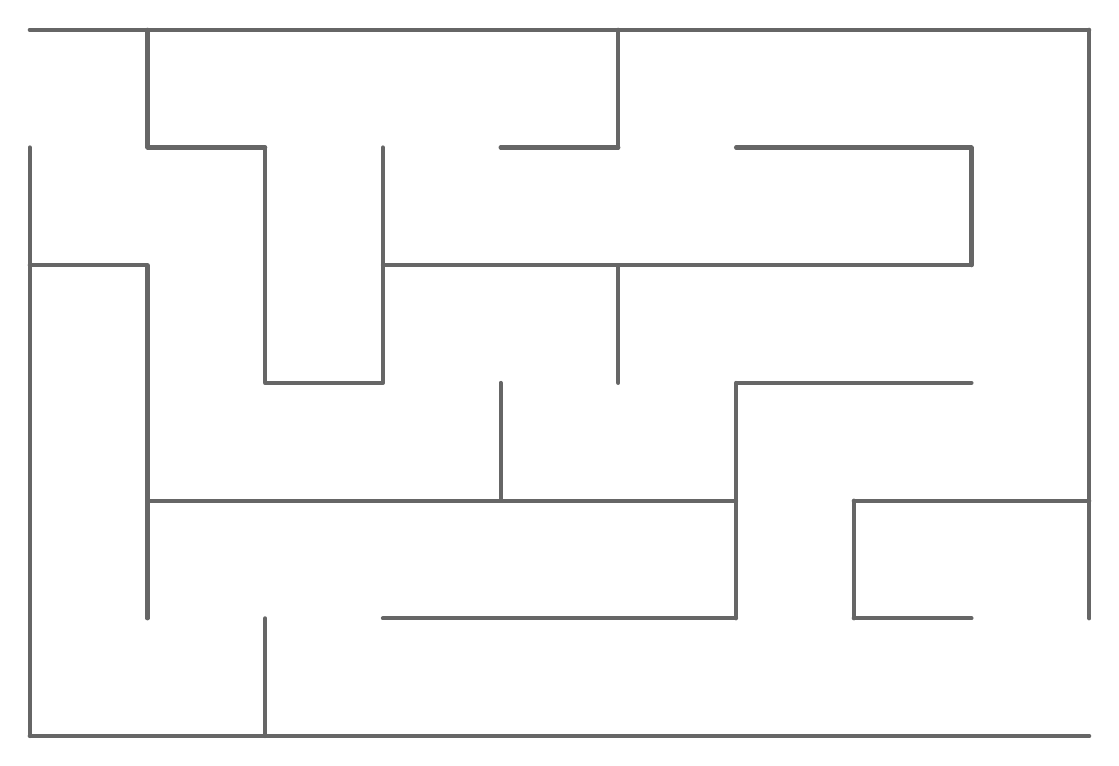
\begin{tikzpicture}[scale=1.3]
        \draw[line width=1.5pt,line cap=round,gray!80!black] (1.15,0.00)--(1.15,-1.15) (5.75,0.00)--(5.75,-1.15) (2.30,-1.15)--(2.30,-2.30) (3.45,-1.15)--(3.45,-2.30) (9.20,-1.15)--(9.20,-2.30) (1.15,-2.30)--(1.15,-3.45) (2.30,-2.30)--(2.30,-3.45) (3.45,-2.30)--(3.45,-3.45) (5.75,-2.30)--(5.75,-3.45) (1.15,-3.45)--(1.15,-4.60) (4.60,-3.45)--(4.60,-4.60) (6.90,-3.45)--(6.90,-4.60) (1.15,-4.60)--(1.15,-5.75) (6.90,-4.60)--(6.90,-5.75) (8.05,-4.60)--(8.05,-5.75) (2.30,-5.75)--(2.30,-6.90) (1.15,-1.15)--(2.30,-1.15) (4.60,-1.15)--(5.75,-1.15) (6.90,-1.15)--(8.05,-1.15) (8.05,-1.15)--(9.20,-1.15) (0.00,-2.30)--(1.15,-2.30) (3.45,-2.30)--(4.60,-2.30) (4.60,-2.30)--(5.75,-2.30) (5.75,-2.30)--(6.90,-2.30) (6.90,-2.30)--(8.05,-2.30) (8.05,-2.30)--(9.20,-2.30) (2.30,-3.45)--(3.45,-3.45) (6.90,-3.45)--(8.05,-3.45) (8.05,-3.45)--(9.20,-3.45) (1.15,-4.60)--(2.30,-4.60) (2.30,-4.60)--(3.45,-4.60) (3.45,-4.60)--(4.60,-4.60) (4.60,-4.60)--(5.75,-4.60) (5.75,-4.60)--(6.90,-4.60) (8.05,-4.60)--(9.20,-4.60) (9.20,-4.60)--(10.35,-4.60) (3.45,-5.75)--(4.60,-5.75) (4.60,-5.75)--(5.75,-5.75) (5.75,-5.75)--(6.90,-5.75) (8.05,-5.75)--(9.20,-5.75) (0.00,0.00)--(10.35,0.00) (0.00,-6.90)--(10.35,-6.90) (0.00,-1.15)--(0.00,-6.90) (10.35,0.00)--(10.35,-5.75);
        \foreach \x/\y in {1.72/-1.72, 2.88/-4.02, 5.17/-2.88, 6.33/-2.88, 8.62/-2.88, 8.62/-4.02, 7.47/-6.33, 8.62/-1.72, 8.62/-5.17, 6.33/-5.17}{\begin{scope}[shift={(\x,\y)}]\OTsao\end{scope}}
        \begin{scope}[shift={(-0.7,-0.58)},scale=1.1]\OTtho\end{scope}
        \begin{scope}[shift={(10.0,-5.75)},scale=1.3]\OTcarot\end{scope}
    \end{tikzpicture}\par}
    \par\medskip
    \noindent Thỏ con nhặt được tất cả \OTo\ ngôi sao trên đường đến chỗ cà rốt. \hfill Có \OTo\ ngôi sao ở các ngõ cụt (không nằm trên đường đi).
\end{bt}

% (đặt trong Buổi 4, trước dòng "--- Hết ---")
% Dùng các lệnh có sẵn: \OTdef, \OTcho, \OTbd, \OTo, \OTforma, \OTcham, màu OT...
%=========================================================

%---------- Hình nhỏ cho trò chơi (vẽ tại gốc tọa độ) ----------
% Chú ong (dài ~0,9cm)
\OTdef\OTong{%
  \filldraw[fill=cyan!20,draw=gray!60,thin] (-0.06,0.2) ellipse (0.11 and 0.19) (0.14,0.21) ellipse (0.1 and 0.17);
  \filldraw[fill=yellow!90!orange,draw=black!70,thin] (0,0) ellipse (0.36 and 0.22);
  \begin{scope}\clip (0,0) ellipse (0.36 and 0.22);
    \fill[black!80] (-0.14,-0.3) rectangle (-0.06,0.3);\fill[black!80] (0.04,-0.3) rectangle (0.12,0.3);\end{scope}
  \filldraw[fill=yellow!90!orange,draw=black!70,thin] (0.38,0.04) circle (0.12);
  \fill (0.42,0.07) circle (0.025);
  \draw[black!70,thin] (0.42,0.15)--(0.5,0.28) (0.35,0.15)--(0.37,0.29);
  \fill[black!80] (-0.38,0) -- (-0.5,0.03) -- (-0.38,-0.03) -- cycle;}
% Tổ ong
\OTdef\OTto{%
  \foreach \y/\w in {-0.45/0.5,-0.18/0.46,0.09/0.4,0.34/0.28}{\filldraw[fill=yellow!70!orange,draw=brown!70!black,rounded corners=3pt] (-\w,\y-0.14) rectangle (\w,\y+0.14);}
  \fill[brown!80!black] (0,-0.38) ellipse (0.14 and 0.1);
  \draw[brown!70!black,thin] (0,0.62)--(0,0.7);}
% Chú cá
\OTdef\OTca{%
  \filldraw[fill=orange!85!yellow,draw=orange!50!black,thin] (-0.1,0) ellipse (0.36 and 0.22);
  \filldraw[fill=orange!85!yellow,draw=orange!50!black,thin] (-0.4,0)--(-0.64,0.2)--(-0.64,-0.2)--cycle;
  \fill[white] (0.12,0.06) circle (0.06);\fill (0.14,0.06) circle (0.03);
  \draw[orange!50!black,thin] (-0.02,-0.15) .. controls (0.02,-0.05) .. (-0.02,0.1);}
% Thỏ
\OTdef\OTtho{%
  \foreach \s in {-1,1}{\filldraw[fill=white,draw=gray!60,thin] (0.1*\s+0.02,0.5) ellipse (0.07 and 0.22);\fill[pink!80] (0.1*\s+0.02,0.5) ellipse (0.03 and 0.14);}
  \filldraw[fill=white,draw=gray!60,thin] (0,-0.2) ellipse (0.3 and 0.26);
  \filldraw[fill=white,draw=gray!60,thin] (0.02,0.2) circle (0.2);
  \fill (-0.05,0.24) circle (0.025) (0.1,0.24) circle (0.025);
  \fill[pink!90!red] (0.02,0.16) circle (0.03);
  \filldraw[fill=white,draw=gray!60,thin] (-0.33,-0.25) circle (0.08);}
% Củ cà rốt
\OTdef\OTcarot{%
  \filldraw[fill=orange,draw=orange!60!black,thin] (-0.14,0.2)--(0.14,0.2)--(0,-0.4)--cycle;
  \draw[orange!60!black,very thin] (-0.07,0.1)--(0.03,0.1) (-0.04,-0.05)--(0.04,-0.05);
  \fill[green!55!black] (0,0.2) .. controls (-0.15,0.35) .. (-0.12,0.5) .. controls (-0.04,0.38) .. cycle;
  \fill[green!55!black] (0,0.2) .. controls (0.15,0.35) .. (0.12,0.5) .. controls (0.04,0.38) .. cycle;
  \fill[green!45!black] (0,0.2) .. controls (-0.04,0.4) .. (0,0.55) .. controls (0.04,0.4) .. cycle;}
% Ngôi sao vàng nhỏ
\OTdef\OTsao{\node[star,star points=5,star point ratio=2.3,inner sep=0pt,minimum size=0.4cm,draw=orange!70!black,fill=yellow,line width=0.4pt] at (0,0) {};}
% Lưới ô: \OTluoi{số cột}{rộng cm}{cao cm}{danh sách ô (theo hàng, từ trên xuống)}
\OTdef\OTluoi[4]{%
  \foreach \t [count=\k] in {#4}{%
    \pgfmathtruncatemacro{\cc}{mod(\k-1,#1)}\pgfmathtruncatemacro{\rr}{div(\k-1,#1)}%
    \node[draw=gray!70,fill=OTkem,rounded corners=4pt,line width=0.6pt,minimum width=#2cm,minimum height=#3cm,inner sep=0pt,font=\large] at ({#2*\cc},{-#3*\rr}) {\t};}}

%%%%%%%%%%%%%%%%%%%%%%%%%%%%%%%%%%%%%%%%%%%%%%%%%%%%%%%%%%
% Bài: đếm hình trong ngôi nhà
%%%%%%%%%%%%%%%%%%%%%%%%%%%%%%%%%%%%%%%%%%%%%%%%%%%%%%%%%%
\OTcho{7cm}\begin{bt}
    Đếm số hình trong bức tranh ngôi nhà rồi điền vào bảng.
    \OTbd{\centering
    \begin{tikzpicture}[scale=1.15]
        % nền cỏ
        \fill[green!35!white] (-0.6,-0.25) rectangle (5.9,0);
        \draw[green!50!black,thick] (-0.6,0)--(5.9,0);
        % ống khói (hình chữ nhật), vẽ trước mái
        \filldraw[fill=red!35!gray!60,draw=gray!70!black,thick] (1.75,2.9) rectangle (2.15,3.75);
        % thân nhà (hình vuông)
        \filldraw[fill=yellow!35!white,draw=brown!70!black,thick] (0,0) rectangle (2.4,2.4);
        % mái nhà (hình tam giác)
        \filldraw[fill=red!75!orange,draw=red!50!black,thick] (-0.2,2.4)--(1.2,3.6)--(2.6,2.4)--cycle;
        % cửa sổ tròn ở mái
        \filldraw[fill=cyan!25!white,draw=gray!70!black,thick] (1.2,2.95) circle (0.28);
        \draw[gray!70!black] (1.2,2.67)--(1.2,3.23) (0.92,2.95)--(1.48,2.95);
        % cửa ra vào (hình chữ nhật)
        \filldraw[fill=brown!60!orange,draw=brown!70!black,thick] (0.3,0) rectangle (0.9,1.3);
        \fill[yellow] (0.78,0.65) circle (0.04);
        % hai cửa sổ (hình vuông)
        \foreach \y in {0.6,1.5}{\filldraw[fill=cyan!25!white,draw=gray!70!black,thick] (1.3,\y) rectangle (2.0,\y+0.7);
          \draw[gray!70!black] (1.65,\y)--(1.65,\y+0.7) (1.3,\y+0.35)--(2.0,\y+0.35);}
        % cây (tam giác + chữ nhật)
        \filldraw[fill=brown!70!black!80,draw=brown!70!black,thick] (4.2,0) rectangle (4.6,1.0);
        \filldraw[fill=green!60!black!80,draw=green!40!black,thick] (3.6,1.0)--(5.2,1.0)--(4.4,2.8)--cycle;
        % mặt trời (hình tròn)
        \foreach \a in {0,30,...,330}{\draw[orange!80!yellow,thick,line cap=round] (4.7,3.8)+(\a:0.55)--+(\a:0.75);}
        \filldraw[fill=yellow,draw=orange!70!black,thick] (4.7,3.8) circle (0.45);
        % bảng thống kê
        \begin{scope}[shift={(6.8,3.3)}]
            \fill[OTnen] (0,0) rectangle (4.9,-0.65);
            \draw[line width=0.5pt] (0,0) rectangle (4.9,-3.05);
            \draw[line width=0.5pt] (2.4,0)--(2.4,-3.05);
            \foreach \i in {1,2,3,4}{\draw[line width=0.5pt] (0,-0.65-0.6*\i+0.6)--(4.9,-0.65-0.6*\i+0.6);}
            \node[font=\bfseries\small] at (1.2,-0.33) {Hình}; \node[font=\bfseries\small] at (3.65,-0.33) {Số lượng};
            \begin{scope}[shift={(1.2,-0.95)}]\filldraw[fill=gray!15,draw=gray!70] (0,0) circle (0.22);\end{scope}
            \begin{scope}[shift={(1.2,-1.55)}]\filldraw[fill=gray!15,draw=gray!70] (-0.22,-0.2) rectangle (0.22,0.24);\end{scope}
            \begin{scope}[shift={(1.2,-2.15)}]\filldraw[fill=gray!15,draw=gray!70] (-0.27,-0.2)--(0.27,-0.2)--(0,0.25)--cycle;\end{scope}
            \begin{scope}[shift={(1.2,-2.75)}]\filldraw[fill=gray!15,draw=gray!70] (-0.33,-0.17) rectangle (0.33,0.17);\end{scope}
        \end{scope}
    \end{tikzpicture}\par}
\end{bt}

%%%%%%%%%%%%%%%%%%%%%%%%%%%%%%%%%%%%%%%%%%%%%%%%%%%%%%%%%%
% Trò chơi 1: mê cung phép tính - giúp ong về tổ
%%%%%%%%%%%%%%%%%%%%%%%%%%%%%%%%%%%%%%%%%%%%%%%%%%%%%%%%%%
\OTcho{8.5cm}\begin{bt}
    \textbf{Trò chơi: Giúp ong về tổ.} Ong con chỉ bay qua những ô có kết quả bằng \textbf{12}. Em hãy tính nhẩm rồi tô màu đường bay của ong con về tổ nhé!
    \OTbd{\centering
    \begin{tikzpicture}
        \OTluoi{6}{2.15}{1.3}{{8+5},{14--3},{9+4},{18--6},{10+2},{17--5},
                              {5+7},{20--8},{16--5},{4+8},{6+7},{13--2},
                              {7+8},{9+3},{6+6},{15--3},{17--4},{5+9},
                              {18--5},{11+3},{15--6},{12+2},{19--8},{4+7}}
        \begin{scope}[shift={(-2.1,-1.3)},scale=1.5]\OTong\end{scope}
        \node[font=\bfseries\small] at (-2.1,-1.95) {Ong con};
        \begin{scope}[shift={(12.8,0)},scale=1.3]\OTto\end{scope}
        \node[font=\bfseries\small] at (12.8,-1.15) {Tổ ong};
    \end{tikzpicture}\par}
\end{bt}

%%%%%%%%%%%%%%%%%%%%%%%%%%%%%%%%%%%%%%%%%%%%%%%%%%%%%%%%%%
% Trò chơi 2: mê cung số tròn chục - cá con về biển
%%%%%%%%%%%%%%%%%%%%%%%%%%%%%%%%%%%%%%%%%%%%%%%%%%%%%%%%%%
\OTcho{7.5cm}\begin{bt}
    \textbf{Trò chơi: Cá con tìm kho báu.} Cá con bơi qua các ô ghi số tròn chục, đi theo thứ tự từ \textbf{bé đến lớn} (10, 20, 30, \ldots). Em hãy vẽ đường bơi giúp cá con nhé!
    \OTbd{\centering
    \begin{tikzpicture}
        \OTluoi{5}{2.3}{1.2}{{10},{20},{30},{12},{45},
                             {27},{63},{40},{50},{60},
                             {31},{58},{86},{19},{70},
                             {74},{9},{100},{90},{80}}
        \begin{scope}[shift={(-2.1,0)},scale=1.5]\OTca\end{scope}
        \node[font=\bfseries\small] at (-2.1,-0.7) {Cá con};
        \begin{scope}[shift={(4.6,-4.85)}]
            \node[star,star points=5,star point ratio=2.2,inner sep=0pt,minimum size=0.9cm,draw=orange!70!black,fill=yellow,line width=0.6pt] at (0,0) {};
            \node[font=\bfseries\small] at (0,-0.7) {Kho báu};
        \end{scope}
    \end{tikzpicture}\par}
\end{bt}

%%%%%%%%%%%%%%%%%%%%%%%%%%%%%%%%%%%%%%%%%%%%%%%%%%%%%%%%%%
% Trò chơi 3: mê cung thỏ tìm cà rốt, nhặt sao
%%%%%%%%%%%%%%%%%%%%%%%%%%%%%%%%%%%%%%%%%%%%%%%%%%%%%%%%%%
\OTcho{10cm}\begin{bt}
    \textbf{Trò chơi: Thỏ con tìm cà rốt.} Em hãy vẽ đường đi giúp thỏ con đến chỗ cà rốt. Trên đường đi, thỏ nhặt được những ngôi sao nào? Hãy đếm và điền số.
    \OTbd{\centering
    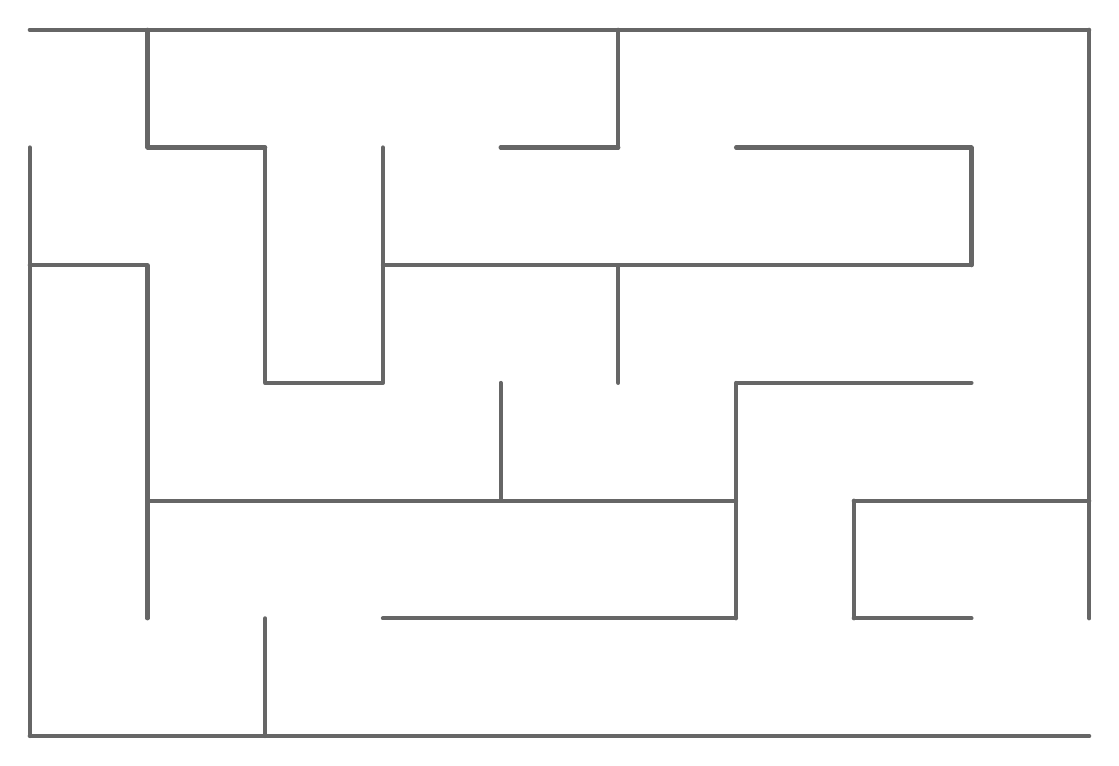
\begin{tikzpicture}[scale=1.3]
        \draw[line width=1.5pt,line cap=round,gray!80!black] (1.15,0.00)--(1.15,-1.15) (5.75,0.00)--(5.75,-1.15) (2.30,-1.15)--(2.30,-2.30) (3.45,-1.15)--(3.45,-2.30) (9.20,-1.15)--(9.20,-2.30) (1.15,-2.30)--(1.15,-3.45) (2.30,-2.30)--(2.30,-3.45) (3.45,-2.30)--(3.45,-3.45) (5.75,-2.30)--(5.75,-3.45) (1.15,-3.45)--(1.15,-4.60) (4.60,-3.45)--(4.60,-4.60) (6.90,-3.45)--(6.90,-4.60) (1.15,-4.60)--(1.15,-5.75) (6.90,-4.60)--(6.90,-5.75) (8.05,-4.60)--(8.05,-5.75) (2.30,-5.75)--(2.30,-6.90) (1.15,-1.15)--(2.30,-1.15) (4.60,-1.15)--(5.75,-1.15) (6.90,-1.15)--(8.05,-1.15) (8.05,-1.15)--(9.20,-1.15) (0.00,-2.30)--(1.15,-2.30) (3.45,-2.30)--(4.60,-2.30) (4.60,-2.30)--(5.75,-2.30) (5.75,-2.30)--(6.90,-2.30) (6.90,-2.30)--(8.05,-2.30) (8.05,-2.30)--(9.20,-2.30) (2.30,-3.45)--(3.45,-3.45) (6.90,-3.45)--(8.05,-3.45) (8.05,-3.45)--(9.20,-3.45) (1.15,-4.60)--(2.30,-4.60) (2.30,-4.60)--(3.45,-4.60) (3.45,-4.60)--(4.60,-4.60) (4.60,-4.60)--(5.75,-4.60) (5.75,-4.60)--(6.90,-4.60) (8.05,-4.60)--(9.20,-4.60) (9.20,-4.60)--(10.35,-4.60) (3.45,-5.75)--(4.60,-5.75) (4.60,-5.75)--(5.75,-5.75) (5.75,-5.75)--(6.90,-5.75) (8.05,-5.75)--(9.20,-5.75) (0.00,0.00)--(10.35,0.00) (0.00,-6.90)--(10.35,-6.90) (0.00,-1.15)--(0.00,-6.90) (10.35,0.00)--(10.35,-5.75);
        \foreach \x/\y in {1.72/-1.72, 2.88/-4.02, 5.17/-2.88, 6.33/-2.88, 8.62/-2.88, 8.62/-4.02, 7.47/-6.33, 8.62/-1.72, 8.62/-5.17, 6.33/-5.17}{\begin{scope}[shift={(\x,\y)}]\OTsao\end{scope}}
        \begin{scope}[shift={(-0.7,-0.58)},scale=1.1]\OTtho\end{scope}
        \begin{scope}[shift={(10.0,-5.75)},scale=1.3]\OTcarot\end{scope}
    \end{tikzpicture}\par}
    \par\medskip
    \noindent Thỏ con nhặt được tất cả \OTo\ ngôi sao trên đường đến chỗ cà rốt. \hfill Có \OTo\ ngôi sao ở các ngõ cụt (không nằm trên đường đi).
\end{bt}

% (đặt trong Buổi 4, trước dòng "--- Hết ---")
% Dùng các lệnh có sẵn: \OTdef, \OTcho, \OTbd, \OTo, \OTforma, \OTcham, màu OT...
%=========================================================

%---------- Hình nhỏ cho trò chơi (vẽ tại gốc tọa độ) ----------
% Chú ong (dài ~0,9cm)
\OTdef\OTong{%
  \filldraw[fill=cyan!20,draw=gray!60,thin] (-0.06,0.2) ellipse (0.11 and 0.19) (0.14,0.21) ellipse (0.1 and 0.17);
  \filldraw[fill=yellow!90!orange,draw=black!70,thin] (0,0) ellipse (0.36 and 0.22);
  \begin{scope}\clip (0,0) ellipse (0.36 and 0.22);
    \fill[black!80] (-0.14,-0.3) rectangle (-0.06,0.3);\fill[black!80] (0.04,-0.3) rectangle (0.12,0.3);\end{scope}
  \filldraw[fill=yellow!90!orange,draw=black!70,thin] (0.38,0.04) circle (0.12);
  \fill (0.42,0.07) circle (0.025);
  \draw[black!70,thin] (0.42,0.15)--(0.5,0.28) (0.35,0.15)--(0.37,0.29);
  \fill[black!80] (-0.38,0) -- (-0.5,0.03) -- (-0.38,-0.03) -- cycle;}
% Tổ ong
\OTdef\OTto{%
  \foreach \y/\w in {-0.45/0.5,-0.18/0.46,0.09/0.4,0.34/0.28}{\filldraw[fill=yellow!70!orange,draw=brown!70!black,rounded corners=3pt] (-\w,\y-0.14) rectangle (\w,\y+0.14);}
  \fill[brown!80!black] (0,-0.38) ellipse (0.14 and 0.1);
  \draw[brown!70!black,thin] (0,0.62)--(0,0.7);}
% Chú cá
\OTdef\OTca{%
  \filldraw[fill=orange!85!yellow,draw=orange!50!black,thin] (-0.1,0) ellipse (0.36 and 0.22);
  \filldraw[fill=orange!85!yellow,draw=orange!50!black,thin] (-0.4,0)--(-0.64,0.2)--(-0.64,-0.2)--cycle;
  \fill[white] (0.12,0.06) circle (0.06);\fill (0.14,0.06) circle (0.03);
  \draw[orange!50!black,thin] (-0.02,-0.15) .. controls (0.02,-0.05) .. (-0.02,0.1);}
% Thỏ
\OTdef\OTtho{%
  \foreach \s in {-1,1}{\filldraw[fill=white,draw=gray!60,thin] (0.1*\s+0.02,0.5) ellipse (0.07 and 0.22);\fill[pink!80] (0.1*\s+0.02,0.5) ellipse (0.03 and 0.14);}
  \filldraw[fill=white,draw=gray!60,thin] (0,-0.2) ellipse (0.3 and 0.26);
  \filldraw[fill=white,draw=gray!60,thin] (0.02,0.2) circle (0.2);
  \fill (-0.05,0.24) circle (0.025) (0.1,0.24) circle (0.025);
  \fill[pink!90!red] (0.02,0.16) circle (0.03);
  \filldraw[fill=white,draw=gray!60,thin] (-0.33,-0.25) circle (0.08);}
% Củ cà rốt
\OTdef\OTcarot{%
  \filldraw[fill=orange,draw=orange!60!black,thin] (-0.14,0.2)--(0.14,0.2)--(0,-0.4)--cycle;
  \draw[orange!60!black,very thin] (-0.07,0.1)--(0.03,0.1) (-0.04,-0.05)--(0.04,-0.05);
  \fill[green!55!black] (0,0.2) .. controls (-0.15,0.35) .. (-0.12,0.5) .. controls (-0.04,0.38) .. cycle;
  \fill[green!55!black] (0,0.2) .. controls (0.15,0.35) .. (0.12,0.5) .. controls (0.04,0.38) .. cycle;
  \fill[green!45!black] (0,0.2) .. controls (-0.04,0.4) .. (0,0.55) .. controls (0.04,0.4) .. cycle;}
% Ngôi sao vàng nhỏ
\OTdef\OTsao{\node[star,star points=5,star point ratio=2.3,inner sep=0pt,minimum size=0.4cm,draw=orange!70!black,fill=yellow,line width=0.4pt] at (0,0) {};}
% Lưới ô: \OTluoi{số cột}{rộng cm}{cao cm}{danh sách ô (theo hàng, từ trên xuống)}
\OTdef\OTluoi[4]{%
  \foreach \t [count=\k] in {#4}{%
    \pgfmathtruncatemacro{\cc}{mod(\k-1,#1)}\pgfmathtruncatemacro{\rr}{div(\k-1,#1)}%
    \node[draw=gray!70,fill=OTkem,rounded corners=4pt,line width=0.6pt,minimum width=#2cm,minimum height=#3cm,inner sep=0pt,font=\large] at ({#2*\cc},{-#3*\rr}) {\t};}}

%%%%%%%%%%%%%%%%%%%%%%%%%%%%%%%%%%%%%%%%%%%%%%%%%%%%%%%%%%
% Bài: đếm hình trong ngôi nhà
%%%%%%%%%%%%%%%%%%%%%%%%%%%%%%%%%%%%%%%%%%%%%%%%%%%%%%%%%%
\OTcho{7cm}\begin{bt}
    Đếm số hình trong bức tranh ngôi nhà rồi điền vào bảng.
    \OTbd{\centering
    \begin{tikzpicture}[scale=1.15]
        % nền cỏ
        \fill[green!35!white] (-0.6,-0.25) rectangle (5.9,0);
        \draw[green!50!black,thick] (-0.6,0)--(5.9,0);
        % ống khói (hình chữ nhật), vẽ trước mái
        \filldraw[fill=red!35!gray!60,draw=gray!70!black,thick] (1.75,2.9) rectangle (2.15,3.75);
        % thân nhà (hình vuông)
        \filldraw[fill=yellow!35!white,draw=brown!70!black,thick] (0,0) rectangle (2.4,2.4);
        % mái nhà (hình tam giác)
        \filldraw[fill=red!75!orange,draw=red!50!black,thick] (-0.2,2.4)--(1.2,3.6)--(2.6,2.4)--cycle;
        % cửa sổ tròn ở mái
        \filldraw[fill=cyan!25!white,draw=gray!70!black,thick] (1.2,2.95) circle (0.28);
        \draw[gray!70!black] (1.2,2.67)--(1.2,3.23) (0.92,2.95)--(1.48,2.95);
        % cửa ra vào (hình chữ nhật)
        \filldraw[fill=brown!60!orange,draw=brown!70!black,thick] (0.3,0) rectangle (0.9,1.3);
        \fill[yellow] (0.78,0.65) circle (0.04);
        % hai cửa sổ (hình vuông)
        \foreach \y in {0.6,1.5}{\filldraw[fill=cyan!25!white,draw=gray!70!black,thick] (1.3,\y) rectangle (2.0,\y+0.7);
          \draw[gray!70!black] (1.65,\y)--(1.65,\y+0.7) (1.3,\y+0.35)--(2.0,\y+0.35);}
        % cây (tam giác + chữ nhật)
        \filldraw[fill=brown!70!black!80,draw=brown!70!black,thick] (4.2,0) rectangle (4.6,1.0);
        \filldraw[fill=green!60!black!80,draw=green!40!black,thick] (3.6,1.0)--(5.2,1.0)--(4.4,2.8)--cycle;
        % mặt trời (hình tròn)
        \foreach \a in {0,30,...,330}{\draw[orange!80!yellow,thick,line cap=round] (4.7,3.8)+(\a:0.55)--+(\a:0.75);}
        \filldraw[fill=yellow,draw=orange!70!black,thick] (4.7,3.8) circle (0.45);
        % bảng thống kê
        \begin{scope}[shift={(6.8,3.3)}]
            \fill[OTnen] (0,0) rectangle (4.9,-0.65);
            \draw[line width=0.5pt] (0,0) rectangle (4.9,-3.05);
            \draw[line width=0.5pt] (2.4,0)--(2.4,-3.05);
            \foreach \i in {1,2,3,4}{\draw[line width=0.5pt] (0,-0.65-0.6*\i+0.6)--(4.9,-0.65-0.6*\i+0.6);}
            \node[font=\bfseries\small] at (1.2,-0.33) {Hình}; \node[font=\bfseries\small] at (3.65,-0.33) {Số lượng};
            \begin{scope}[shift={(1.2,-0.95)}]\filldraw[fill=gray!15,draw=gray!70] (0,0) circle (0.22);\end{scope}
            \begin{scope}[shift={(1.2,-1.55)}]\filldraw[fill=gray!15,draw=gray!70] (-0.22,-0.2) rectangle (0.22,0.24);\end{scope}
            \begin{scope}[shift={(1.2,-2.15)}]\filldraw[fill=gray!15,draw=gray!70] (-0.27,-0.2)--(0.27,-0.2)--(0,0.25)--cycle;\end{scope}
            \begin{scope}[shift={(1.2,-2.75)}]\filldraw[fill=gray!15,draw=gray!70] (-0.33,-0.17) rectangle (0.33,0.17);\end{scope}
        \end{scope}
    \end{tikzpicture}\par}
\end{bt}

%%%%%%%%%%%%%%%%%%%%%%%%%%%%%%%%%%%%%%%%%%%%%%%%%%%%%%%%%%
% Trò chơi 1: mê cung phép tính - giúp ong về tổ
%%%%%%%%%%%%%%%%%%%%%%%%%%%%%%%%%%%%%%%%%%%%%%%%%%%%%%%%%%
\OTcho{8.5cm}\begin{bt}
    \textbf{Trò chơi: Giúp ong về tổ.} Ong con chỉ bay qua những ô có kết quả bằng \textbf{12}. Em hãy tính nhẩm rồi tô màu đường bay của ong con về tổ nhé!
    \OTbd{\centering
    \begin{tikzpicture}
        \OTluoi{6}{2.15}{1.3}{{8+5},{14--3},{9+4},{18--6},{10+2},{17--5},
                              {5+7},{20--8},{16--5},{4+8},{6+7},{13--2},
                              {7+8},{9+3},{6+6},{15--3},{17--4},{5+9},
                              {18--5},{11+3},{15--6},{12+2},{19--8},{4+7}}
        \begin{scope}[shift={(-2.1,-1.3)},scale=1.5]\OTong\end{scope}
        \node[font=\bfseries\small] at (-2.1,-1.95) {Ong con};
        \begin{scope}[shift={(12.8,0)},scale=1.3]\OTto\end{scope}
        \node[font=\bfseries\small] at (12.8,-1.15) {Tổ ong};
    \end{tikzpicture}\par}
\end{bt}

%%%%%%%%%%%%%%%%%%%%%%%%%%%%%%%%%%%%%%%%%%%%%%%%%%%%%%%%%%
% Trò chơi 2: mê cung số tròn chục - cá con về biển
%%%%%%%%%%%%%%%%%%%%%%%%%%%%%%%%%%%%%%%%%%%%%%%%%%%%%%%%%%
\OTcho{7.5cm}\begin{bt}
    \textbf{Trò chơi: Cá con tìm kho báu.} Cá con bơi qua các ô ghi số tròn chục, đi theo thứ tự từ \textbf{bé đến lớn} (10, 20, 30, \ldots). Em hãy vẽ đường bơi giúp cá con nhé!
    \OTbd{\centering
    \begin{tikzpicture}
        \OTluoi{5}{2.3}{1.2}{{10},{20},{30},{12},{45},
                             {27},{63},{40},{50},{60},
                             {31},{58},{86},{19},{70},
                             {74},{9},{100},{90},{80}}
        \begin{scope}[shift={(-2.1,0)},scale=1.5]\OTca\end{scope}
        \node[font=\bfseries\small] at (-2.1,-0.7) {Cá con};
        \begin{scope}[shift={(4.6,-4.85)}]
            \node[star,star points=5,star point ratio=2.2,inner sep=0pt,minimum size=0.9cm,draw=orange!70!black,fill=yellow,line width=0.6pt] at (0,0) {};
            \node[font=\bfseries\small] at (0,-0.7) {Kho báu};
        \end{scope}
    \end{tikzpicture}\par}
\end{bt}

%%%%%%%%%%%%%%%%%%%%%%%%%%%%%%%%%%%%%%%%%%%%%%%%%%%%%%%%%%
% Trò chơi 3: mê cung thỏ tìm cà rốt, nhặt sao
%%%%%%%%%%%%%%%%%%%%%%%%%%%%%%%%%%%%%%%%%%%%%%%%%%%%%%%%%%
\OTcho{10cm}\begin{bt}
    \textbf{Trò chơi: Thỏ con tìm cà rốt.} Em hãy vẽ đường đi giúp thỏ con đến chỗ cà rốt. Trên đường đi, thỏ nhặt được những ngôi sao nào? Hãy đếm và điền số.
    \OTbd{\centering
    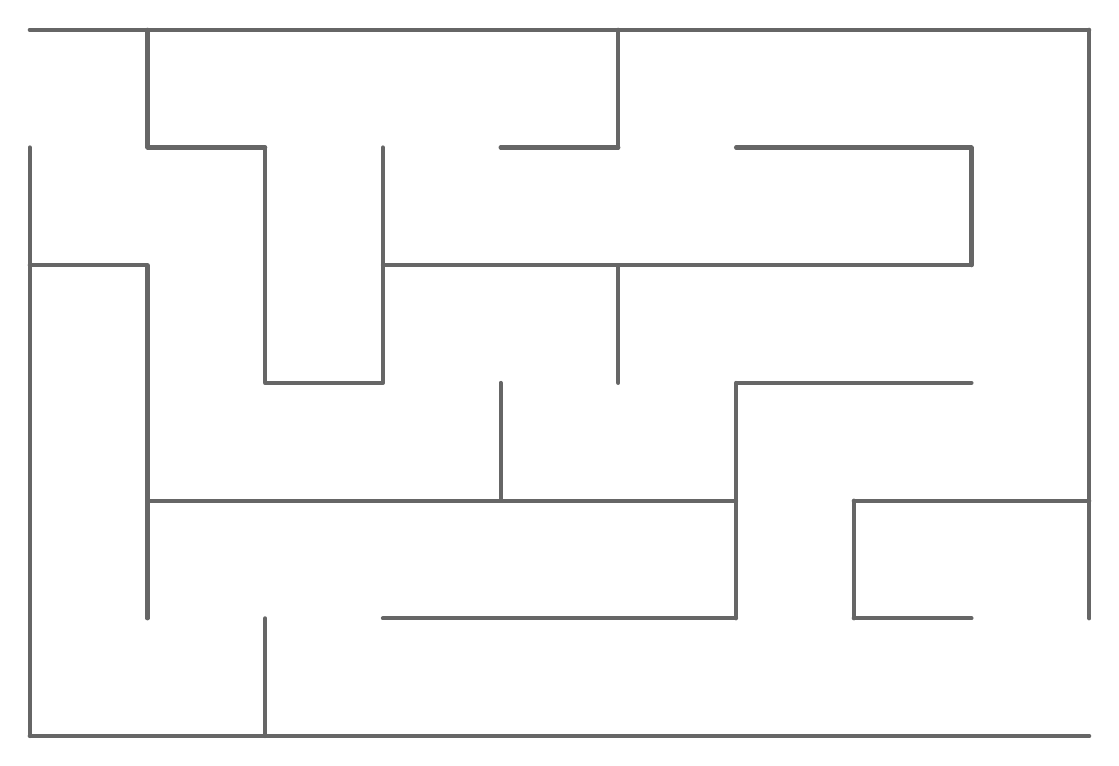
\begin{tikzpicture}[scale=1.3]
        \draw[line width=1.5pt,line cap=round,gray!80!black] (1.15,0.00)--(1.15,-1.15) (5.75,0.00)--(5.75,-1.15) (2.30,-1.15)--(2.30,-2.30) (3.45,-1.15)--(3.45,-2.30) (9.20,-1.15)--(9.20,-2.30) (1.15,-2.30)--(1.15,-3.45) (2.30,-2.30)--(2.30,-3.45) (3.45,-2.30)--(3.45,-3.45) (5.75,-2.30)--(5.75,-3.45) (1.15,-3.45)--(1.15,-4.60) (4.60,-3.45)--(4.60,-4.60) (6.90,-3.45)--(6.90,-4.60) (1.15,-4.60)--(1.15,-5.75) (6.90,-4.60)--(6.90,-5.75) (8.05,-4.60)--(8.05,-5.75) (2.30,-5.75)--(2.30,-6.90) (1.15,-1.15)--(2.30,-1.15) (4.60,-1.15)--(5.75,-1.15) (6.90,-1.15)--(8.05,-1.15) (8.05,-1.15)--(9.20,-1.15) (0.00,-2.30)--(1.15,-2.30) (3.45,-2.30)--(4.60,-2.30) (4.60,-2.30)--(5.75,-2.30) (5.75,-2.30)--(6.90,-2.30) (6.90,-2.30)--(8.05,-2.30) (8.05,-2.30)--(9.20,-2.30) (2.30,-3.45)--(3.45,-3.45) (6.90,-3.45)--(8.05,-3.45) (8.05,-3.45)--(9.20,-3.45) (1.15,-4.60)--(2.30,-4.60) (2.30,-4.60)--(3.45,-4.60) (3.45,-4.60)--(4.60,-4.60) (4.60,-4.60)--(5.75,-4.60) (5.75,-4.60)--(6.90,-4.60) (8.05,-4.60)--(9.20,-4.60) (9.20,-4.60)--(10.35,-4.60) (3.45,-5.75)--(4.60,-5.75) (4.60,-5.75)--(5.75,-5.75) (5.75,-5.75)--(6.90,-5.75) (8.05,-5.75)--(9.20,-5.75) (0.00,0.00)--(10.35,0.00) (0.00,-6.90)--(10.35,-6.90) (0.00,-1.15)--(0.00,-6.90) (10.35,0.00)--(10.35,-5.75);
        \foreach \x/\y in {1.72/-1.72, 2.88/-4.02, 5.17/-2.88, 6.33/-2.88, 8.62/-2.88, 8.62/-4.02, 7.47/-6.33, 8.62/-1.72, 8.62/-5.17, 6.33/-5.17}{\begin{scope}[shift={(\x,\y)}]\OTsao\end{scope}}
        \begin{scope}[shift={(-0.7,-0.58)},scale=1.1]\OTtho\end{scope}
        \begin{scope}[shift={(10.0,-5.75)},scale=1.3]\OTcarot\end{scope}
    \end{tikzpicture}\par}
    \par\medskip
    \noindent Thỏ con nhặt được tất cả \OTo\ ngôi sao trên đường đến chỗ cà rốt. \hfill Có \OTo\ ngôi sao ở các ngõ cụt (không nằm trên đường đi).
\end{bt}
